
\documentclass[aspectratio=169,11pt]{beamer}

% ---------- Theme ----------
\usetheme{Madrid}
\usecolortheme{default}
\setbeamertemplate{navigation symbols}{}
\setbeamertemplate{footline}{
  \leavevmode%
  \hbox{%
  \begin{beamercolorbox}[wd=.78\paperwidth,ht=2.6ex,dp=1ex,leftskip=1em]{author in head/foot}%
    \color{gray!80}\small Sayona C Sajan \hspace{0.8em}|\hspace{0.8em} Mathematics for Computing
  \end{beamercolorbox}%
  \begin{beamercolorbox}[wd=.22\paperwidth,ht=2.6ex,dp=1ex,center]{date in head/foot}%
    \color{gray!80}\small \insertframenumber/\inserttotalframenumber
  \end{beamercolorbox}}%
}

% ---------- Packages ----------
\usepackage{amsmath,amssymb,mathtools}
\usepackage{tikz}
\usetikzlibrary{arrows.meta,positioning,calc,shapes.geometric}
\usepackage{booktabs}
\usepackage{array}
\usepackage{ragged2e}

% ---------- Colors ----------
\definecolor{navy}{RGB}{23,43,77}
\definecolor{teal}{RGB}{28,126,140}
\definecolor{mint}{RGB}{224,245,242}
\definecolor{gold}{RGB}{229,174,64}
\definecolor{ink}{RGB}{38,48,60}
\definecolor{paper}{RGB}{247,249,252}

\setbeamercolor{normal text}{fg=ink,bg=paper}
\setbeamercolor{structure}{fg=teal}
\setbeamercolor{frametitle}{fg=navy,bg=paper}
\setbeamercolor{title}{fg=navy}
\setbeamercolor{block title}{fg=white,bg=navy}
\setbeamercolor{block body}{fg=ink,bg=white}
\setbeamercolor{alerted text}{fg=teal}

\setbeamertemplate{frametitle}{
  \vspace{0.25cm}
  \nointerlineskip
  \begin{beamercolorbox}[wd=\paperwidth,leftskip=0.65cm,rightskip=0.65cm,sep=0.15cm]{frametitle}
    \usebeamerfont{frametitle}\insertframetitle
    \hfill
    \tikz\draw[teal,line width=1.5pt] (0,0)--(0.8,0);
  \end{beamercolorbox}
}

% ---------- Subtle geometric background ----------
\setbeamertemplate{background}{
\begin{tikzpicture}[remember picture,overlay]
  \fill[paper] (current page.south west) rectangle (current page.north east);
  \fill[mint,opacity=.38]
    (current page.north west) -- ++(4.3cm,0) -- ++(-1.4cm,-2.2cm) -- cycle;
  \fill[teal!7]
    (current page.south east) -- ++(-5.0cm,0) -- ++(2.0cm,2.5cm) -- cycle;
  \draw[teal!14,line width=.7pt]
    ([xshift=-0.2cm]current page.north east) circle (1.45cm);
  \draw[gold!25,line width=.8pt]
    ([xshift=0.4cm,yshift=0.15cm]current page.south west) circle (1.0cm);
\end{tikzpicture}
}

\setbeamertemplate{blocks}[rounded][shadow=false]
\setlength{\parskip}{3pt}

% ---------- Metadata ----------
\title{Mathematics for Computing}
\subtitle{Assignment 1}
\author{Sayona C Sajan}
\institute{Department of Computer Science and Engineering\\
with Artificial Intelligence and Software Engineering\\
CUSAT}
\date{August 13, 2026}

\newcommand{\examplebox}[2]{
\begin{block}{Example}
\textbf{#1}\\[-1mm]
#2
\end{block}
}

\begin{document}

% 1
\begin{frame}
\titlepage
\end{frame}

% 2
\begin{frame}{Content}
\begin{columns}[T]
\column{.48\textwidth}
\begin{enumerate}
  \item Cardinality of a Set
  \item Types of Sets in Computing
  \item Set-builder Form Examples
  \item Inclusion--Exclusion Principle
\end{enumerate}
\column{.48\textwidth}
\begin{enumerate}\setcounter{enumi}{4}
  \item Partially Ordered Sets (Posets)
  \item Hasse Diagram Examples
  \item Key Takeaways
\end{enumerate}
\end{columns}
\vfill
\centering
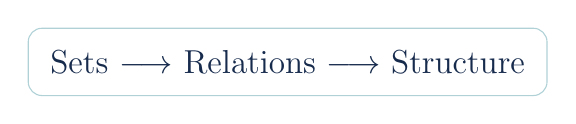
\begin{tikzpicture}
\node[draw=teal!35,fill=white,rounded corners=5pt,inner sep=8pt]
{\large\textcolor{navy}{Sets $\longrightarrow$ Relations $\longrightarrow$ Structure}};
\end{tikzpicture}
\end{frame}

% 3
\begin{frame}{Cardinality of a Set}
\textbf{Cardinality} is the number of distinct elements contained in a set.

\[
|A|=\text{number of elements of }A
\]

\examplebox{A computing-oriented example}{
Let
\[
A=\{\text{CPU},\text{GPU},\text{RAM},\text{SSD},\text{NIC},\text{USB}\}.
\]
There are six distinct components, so
\[
\boxed{|A|=6}.
\]
}
\end{frame}

% 4
\begin{frame}{Types of Sets: Finite Set}
A \textbf{finite set} contains a limited number of elements.

\[
|A|=n,\qquad n\in\mathbb{N}.
\]

\examplebox{Example: network status labels}{
A monitoring system may use
\[
S=\{\text{Online},\text{Idle},\text{Busy},\text{Offline}\}.
\]
The number of possible labels is four, hence $S$ is finite.
}

\[
S=\{x\in U\mid x\text{ is one of the four status labels}\}.
\]
\end{frame}

% 5
\begin{frame}{Types of Sets: Infinite Set}
An \textbf{infinite set} has infinitely many possible elements.

\examplebox{Example: possible latency values}{
If latency is represented by a non-negative real number,
\[
L=\{x\in\mathbb{R}\mid x\ge 0\}.
\]
Between any two different real-valued measurements, more real values can be chosen. Thus $L$ is infinite.
}

\[
L=\{x\in\mathbb{R}\mid x\ge 0\}.
\]
\end{frame}

% 6
\begin{frame}{Types of Sets: Null Set}
A \textbf{null (empty) set} contains no elements and is denoted by $\varnothing$.

\examplebox{Example: unavailable error category}{
Suppose a test run records only errors from the set
\[
E=\{\text{timeout},\text{syntax},\text{memory}\}.
\]
If a particular run contains no memory errors, then
\[
M=\{\text{memory errors observed in the run}\}=\varnothing.
\]
}
\end{frame}

% 7
\begin{frame}{Types of Sets: Countable Set}
A \textbf{countable set} can be listed as a sequence and associated with natural numbers.

\examplebox{Example: packet sequence numbers}{
For a finite capture, packet identifiers can be listed:
\[
P=\{101,102,103,104,105,\ldots\}.
\]
The identifiers can be indexed one after another, so the set is countable.
}

\[
P=\{f(n)\mid n\in\mathbb{N}\}
\]
for an appropriate enumeration function $f$.
\end{frame}

% 8
\begin{frame}{Types of Sets: Power Set}
The \textbf{power set} $\mathcal{P}(A)$ is the set of every subset of $A$, including $\varnothing$ and $A$ itself.

\examplebox{Example: system capabilities}{
Let
\[
C=\{\text{GPS},\text{WiFi},\text{Bluetooth}\}.
\]
Then
\[
\begin{aligned}
\mathcal{P}(C)=\{&
\varnothing,\{\text{GPS}\},\{\text{WiFi}\},\{\text{Bluetooth}\},\\
&\{\text{GPS,WiFi}\},\{\text{GPS,Bluetooth}\},
\{\text{WiFi,Bluetooth}\},C\}.
\end{aligned}
\]
}

\[
\boxed{|\mathcal{P}(C)|=2^{|C|}=2^3=8}.
\]
\end{frame}

% 9
\begin{frame}{Types of Sets: Subset}
A set $T$ is a \textbf{subset} of $D$ if every element of $T$ also belongs to $D$.

\[
T\subseteq D.
\]

\examplebox{Example: selected software tools}{
\[
D=\{\text{Python},\text{Java},\text{C},\text{JavaScript}\},
\quad
T=\{\text{Python},\text{JavaScript}\}.
\]
Every element of $T$ occurs in $D$, therefore
\[
\boxed{T\subseteq D}.
\]
}
\end{frame}

% 10
\begin{frame}{Types of Sets: Equal Set}
Two sets are \textbf{equal} when they contain exactly the same elements, regardless of order.

\examplebox{Example}{
\[
A=\{\text{TCP},\text{UDP},\text{HTTP}\}
\]
and
\[
B=\{\text{HTTP},\text{TCP},\text{UDP}\}.
\]
Since order does not matter for sets,
\[
\boxed{A=B}.
\]
}
\end{frame}

% 11
\begin{frame}{Types of Sets: Equivalent Set}
Two sets are \textbf{equivalent} if they contain the same number of elements.

\examplebox{Example}{
Let
\[
A=\{\text{Linux},\text{Windows},\text{macOS}\}
\]
and
\[
B=\{\text{Java},\text{Python},\text{C++}\}.
\]
Both have three elements:
\[
|A|=|B|=3,
\qquad\therefore\qquad
\boxed{A\sim B}.
\]
}
\end{frame}

% 12
\begin{frame}{Types of Sets: Superset}
A set $D$ is a \textbf{superset} of $T$ when it contains every element of $T$.

\[
D\supseteq T.
\]

\examplebox{Example}{
\[
D=\{\text{HTML},\text{CSS},\text{JavaScript},\text{React}\}
\]
and
\[
T=\{\text{HTML},\text{CSS}\}.
\]
Hence
\[
\boxed{D\supseteq T}.
\]
}
\end{frame}

% 13
\begin{frame}{Types of Sets: Singleton Set}
A \textbf{singleton set} contains exactly one element.

\[
|A|=1.
\]

\examplebox{Example: one active server}{
If only one server is currently selected for deployment,
\[
A=\{\text{server-07}\}.
\]
Therefore $A$ is a singleton set.
}

\[
A=\{x\mid x=a\}.
\]
\end{frame}
\begin{frame}{Set Operations}

Set operations are used to combine or compare sets.

\vspace{0.3cm}

\textbf{1. Union}

The union of $A$ and $B$ contains all elements belonging to $A$ or $B$.

\[
A\cup B=\{x\mid x\in A\text{ or }x\in B\}
\]

\vspace{0.2cm}

\textbf{2. Intersection}

The intersection contains elements common to both sets.

\[
A\cap B=\{x\mid x\in A\text{ and }x\in B\}
\]

\vspace{0.2cm}

\textbf{3. Difference}

The difference $A-B$ contains elements in $A$ but not in $B$.

\[
A-B=\{x\mid x\in A\text{ and }x\notin B\}
\]

\end{frame}
% 15[17:39, 13/08/2026] Haripriya College: \begin{frame}{Set Operations: Complement and Symmetric Difference}

\textbf{4. Complement}

The complement of $A$ contains elements in the universal set $U$
that are not in $A$.

\[
A^c=U-A
\]

\vspace{0.4cm}

\textbf{5. Symmetric Difference}

The symmetric difference contains elements belonging to exactly
one of the two sets.

\[
A\triangle B=(A-B)\cup(B-A)
\]

\vspace{0.4cm}

\begin{block}{Important}
Set operations are useful for organizing, filtering, and comparing
data in computing and data science.
\end{block}

\end{frame}
 \begin{frame}{Set Operations: Computing Example}

Consider two sets of programming languages:

\[
A=\{\text{Python, Java, C}\},
\qquad
B=\{\text{Java, C++, Python}\}
\]

\vspace{0.2cm}

\begin{block}{Union}
\[
A\cup B=\{\text{Python, Java, C, C++}\}
\]
\end{block}

\begin{block}{Intersection}
\[
A\cap B=\{\text{Python, Java}\}
\]
\end{block}

\begin{block}{Difference}
\[
A-B=\{\text{C}\}
\]
\end{block}


\end{frame}
% 14
\begin{frame}{Set-builder Form: Examples I}
\textbf{1. Natural numbers that are multiples of 4 but not 8}
\[
A=\{x\in\mathbb{N}\mid 4\mid x,\;8\nmid x\}.
\]
\[
A=\{4,12,20,28,36,\ldots\}.
\]

\vspace{3mm}
\textbf{2. Perfect fourth powers}
\[
B=\{x\in\mathbb{N}\mid x=n^4,\;n\in\mathbb{N}\}.
\]
\[
B=\{1,16,81,256,625,\ldots\}.
\]
\end{frame}

\begin{frame}{Set-builder Form: Examples II}
\textbf{3. Natural numbers between 12 and 60}
\[
A=\{x\in\mathbb{N}\mid 12<x<60\}.
\]
\[
A=\{13,14,15,\ldots,59\}.
\]

\vspace{3mm}
\textbf{4. Positive integers leaving remainder 2 when divided by 7}
\[
B=\{x\in\mathbb{Z}^+\mid x=7n+2,\;n\in\mathbb{N}_0\}.
\]
\[
B=\{2,9,16,23,30,\ldots\}.
\]
\end{frame}

% 16
\begin{frame}{Set-builder Form: Examples III}
\textbf{5. Even natural numbers from 2 to 20}
\[
A=\{x\in\mathbb{N}\mid x=2n,\;1\le n\le10\}.
\]
\[
A=\{2,4,6,8,10,12,14,16,18,20\}.
\]

\vspace{3mm}
\textbf{6. Factors of 36}
\[
B=\{x\in\mathbb{N}\mid x\mid36\}.
\]
\[
B=\{1,2,3,4,6,9,12,18,36\}.
\]
\end{frame}

% 17
\begin{frame}{Set-builder Form: Examples IV}
\textbf{7. Ordered pairs whose product is 12}
\[
A=\{(x,y)\in\mathbb{Z}^2\mid xy=12\}.
\]
Some positive pairs are
\[
(1,12),(2,6),(3,4),(4,3),(6,2),(12,1).
\]

\vspace{3mm}
\textbf{8. Natural numbers divisible by 4 or 5}
\[
B=\{x\in\mathbb{N}\mid 4\mid x\ \text{or}\ 5\mid x\}.
\]
\[
B=\{4,5,8,10,12,15,16,20,\ldots\}.
\]
\end{frame}

% 18
\begin{frame}{Set-builder Form: Examples V}
\textbf{9. Cubes of natural numbers}
\[
A=\{n^3\mid n\in\mathbb{N}\}.
\]
\[
A=\{1,8,27,64,125,\ldots\}.
\]

\vspace{3mm}
\textbf{10. Prime numbers from 1 to 35}
\[
B=\{x\in\mathbb{N}\mid x\text{ is prime and }1<x\le35\}.
\]
\[
B=\{2,3,5,7,11,13,17,19,23,29,31\}.
\]
\end{frame}

% 19
\begin{frame}{Inclusion--Exclusion Principle}
The \textbf{Inclusion--Exclusion Principle} counts elements in a union while correcting for overlaps.

For three sets:
\[
\boxed{
|A\cup B\cup C|
=|A|+|B|+|C|
-|A\cap B|-|A\cap C|-|B\cap C|
+|A\cap B\cap C|
}
\]

\examplebox{Small numerical example}{
Suppose $|A|=24$, $|B|=18$, and $|A\cap B|=7$. Then
\[
|A\cup B|=24+18-7=\boxed{35}.
\]
The intersection is subtracted because those elements were counted twice.
}
\end{frame}

% 20
\begin{frame}{Partially Ordered Sets (Posets)}
A \textbf{partially ordered set} is a set together with a relation satisfying:

\begin{enumerate}
\item \textbf{Reflexive:} $a\preceq a$.
\item \textbf{Antisymmetric:} if $a\preceq b$ and $b\preceq a$, then $a=b$.
\item \textbf{Transitive:} if $a\preceq b$ and $b\preceq c$, then $a\preceq c$.
\end{enumerate}

\examplebox{Example: divisibility}{
Let
\[
P=\{1,2,4,8\}
\]
with the relation ``divides'' $(\mid)$.
Since $1\mid2$, $2\mid4$, and $4\mid8$, the relation forms a poset.
}
\end{frame}

% 21
\begin{frame}{Hasse Diagram: Divisibility Poset}
Consider
\[
P=\{1,2,4,8\},\qquad \text{relation } \mid.
\]

Only the immediate covering relations are drawn.

\begin{center}
\resizebox{!}{2.65cm}{%
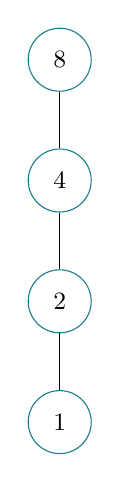
\begin{tikzpicture}[node distance=0.72cm,
  every node/.style={circle,draw=teal,fill=white,minimum size=8mm,font=\small}]
\node (n1) {1};
\node (n2) [above=of n1] {2};
\node (n4) [above=of n2] {4};
\node (n8) [above=of n4] {8};
\draw (n1)--(n2)--(n4)--(n8);
\end{tikzpicture}%
}
\end{center}

Thus $(P,\mid)$ is a partially ordered set.
\end{frame}

% 22
\begin{frame}{Hasse Diagram: Subset Poset}
Let
\[
P=\{\varnothing,\{x\},\{y\},\{x,y\}\}
\]
with relation $\subseteq$.

\begin{center}
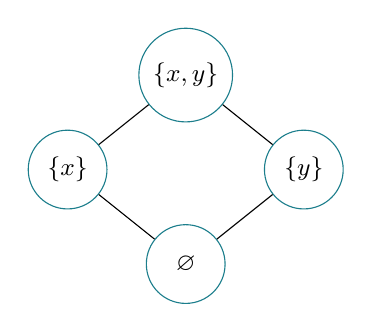
\begin{tikzpicture}[every node/.style={circle,draw=teal,fill=white,minimum size=10mm,font=\small}]
\node (top) at (0,2.4) {$\{x,y\}$};
\node (x) at (-1.5,1.2) {$\{x\}$};
\node (y) at (1.5,1.2) {$\{y\}$};
\node (bot) at (0,0) {$\varnothing$};
\draw (top)--(x) (top)--(y) (x)--(bot) (y)--(bot);
\end{tikzpicture}
\end{center}

The diagram represents the subset relation without drawing transitive edges.
\end{frame}

% 23
\begin{frame}{Hasse Diagram: Factor Poset}
Consider
\[
P=\{1,2,3,6,12,24\}
\]
under divisibility.

The immediate covering relations are
\[
1\mid2,\quad 1\mid3,\quad 2\mid6,\quad 3\mid6,\quad
6\mid12,\quad 12\mid24.
\]

These relations are enough to construct the Hasse diagram.

\begin{center}
\resizebox{!}{3.0cm}{%
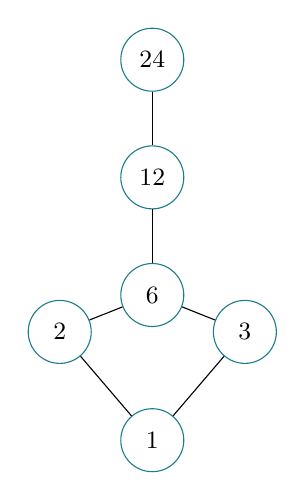
\begin{tikzpicture}[node distance=0.68cm,
  every node/.style={circle,draw=teal,fill=white,minimum size=8mm,font=\small}]
\node (one) {1};
\node (two) [above left=0.8cm and 0.6cm of one] {2};
\node (three) [above right=0.8cm and 0.6cm of one] {3};
\node (six) [above=of one,yshift=0.35cm] {6};
\node (twelve) [above=of six] {12};
\node (twentyfour) [above=of twelve] {24};
\draw (one)--(two);
\draw (one)--(three);
\draw (two)--(six);
\draw (three)--(six);
\draw (six)--(twelve);
\draw (twelve)--(twentyfour);
\end{tikzpicture}%
}
\end{center}
\end{frame}
%------------------------------------------------
\begin{frame}{Chain and Antichain}

\small

\begin{columns}[T]

\begin{column}{0.48\textwidth}

\begin{block}{Chain}

\textbf{Definition:} Every pair of elements is comparable.

\[
a\preceq b\quad\text{or}\quad b\preceq a
\]

\textbf{Example:}

\[
P=\{1,2,4,8\},\qquad C=\{1,2,4\}
\]

Under divisibility,

\[
1\mid2,\quad2\mid4,\quad1\mid4.
\]

Hence,

\[
\boxed{C\text{ is a chain}}
\]

\end{block}

\end{column}


\begin{column}{0.48\textwidth}

\begin{block}{Antichain}

\textbf{Definition:} No two distinct elements are comparable.

\[
a\npreceq b\quad\text{and}\quad b\npreceq a
\]

\textbf{Example:}

\[
P=\{1,2,3,6\},\qquad A=\{2,3\}
\]

Under divisibility,

\[
2\nmid3,\quad3\nmid2.
\]

Hence,

\[
\boxed{A\text{ is an antichain}}
\]

\end{block}

\end{column}

\end{columns}

\end{frame}
%------------------------------------------------
%------------------------------------------------

\end{document}


